%!TEX root = ../main.tex
\chapter{Design}
In this section, I will discuss both aesthetic and technical designs for the application as well as offer an overall design of the system as a whole.

\section{System Design}
In order to gain a better overview of the system, I mapped out how the individual pieces of the KidQuest system work together.

\begin{figure}[ht]
	\centering
	\includegraphics[scale=0.55]{images/SystemDiagram.png}
	\caption{System Design Diagram}
	\label{fig:systemdesign}
\end{figure} 

\subsection{Server API}
As initial designs began it was clear that my initial database/class diagrams were drawn with incorrect assumptions about the project. 
Initial designs attempted to implement all workflows into the applications and communicate directly between two phones, storing all necessary on the client end. 
However, these designs presented many drawbacks, the key of which was that communications between two mobile devices appeared to be unreliable enough to ensure that data remained synchronized between them.
For example, if a child user marked a quest as completed, their phone would send a notification to the parent user.
However if this notification was not received by the parent, the quest would fall into a limbo-like state where the parent is waiting for it to be completed and the child is waiting for it to be confirmed.

Therefore, the system calls for a centralized location in order for two users to reliably communicate between each other.
By implementing the functionality into a server-based application, the system becomes significantly more portable. 
As all functionality of the system rests in a centralized location, any ported apps - such as iOS or a web app - would only have to tie into the existing API.
This would make porting the application trivial, as the only code that would need to be created for these apps would be code to simply send and receive web service requests to the API and display the data that it receives.

It also has a positive effect on the maintainability of the software. 
Updating software on mobile becomes difficult as some people do not always update their apps to the latest version. 
Furthermore, two users working together on two different versions of the app could cause serious interoperability problems.
The server API helps this, as all functionality updates to the system can be made in the server rather than user devices, effectively distributing updated functionality to all users at once, instantly.

However, server-side implementation does have two main consequences which must be considered. 
Firstly, users would now require an internet connection to use the app so that it is able to communicate with the server.
This may cause an issue for users who have limited data plans on their phone contracts or limited connectivity. 
However, this issue can be mitigated by keeping the data sent to a minimum and making the app only send requests it needs to.
Furthermore, options exist in the Android OS that restrict an application's data usage, meaning that requests will be halted until the user has connected to a usable wi-fi network.

Secondly, All users will be required to create an account with the server in order to use the app, as the system needs to store the data on the server end rather than on the users' phone.
I would need to have increased security requirements surrounding that data, making sure that it is sufficiently encrypted during transit between the user device and server, and that the data stored on the server itself is sufficiently protected as well.

\subsubsection{Security Requirements}
To handle logins securely, I plan on implementing a token-based authentication system within the server. 
Upon their first request, the user submits their username and password within a HTTP POST request to the server.
The server then sends back an encrypted token that is derived out of various hashed attributes of their account, which the user client then stores.
The app will then authenticate itself with the server for every future request using this token.
This offers the main benefit that the app only has to store the token and not the username and password, which would leave it vulnerable to other (malicious) apps accessing critical user data.
It will also mean that the app will not have to send their username and password with each request that it makes to the API, minimizing the risk of the password within the request being intercepted in transport.
The password is only stored within the server, which has securely encrypted it with a salted hash.

\section{Database}
\subsection{Design}
Entity Relationship Diagrams (ERD) are a visual representation of tables, columns and relationships within a database.

\begin{figure}[ht]
	\centering
	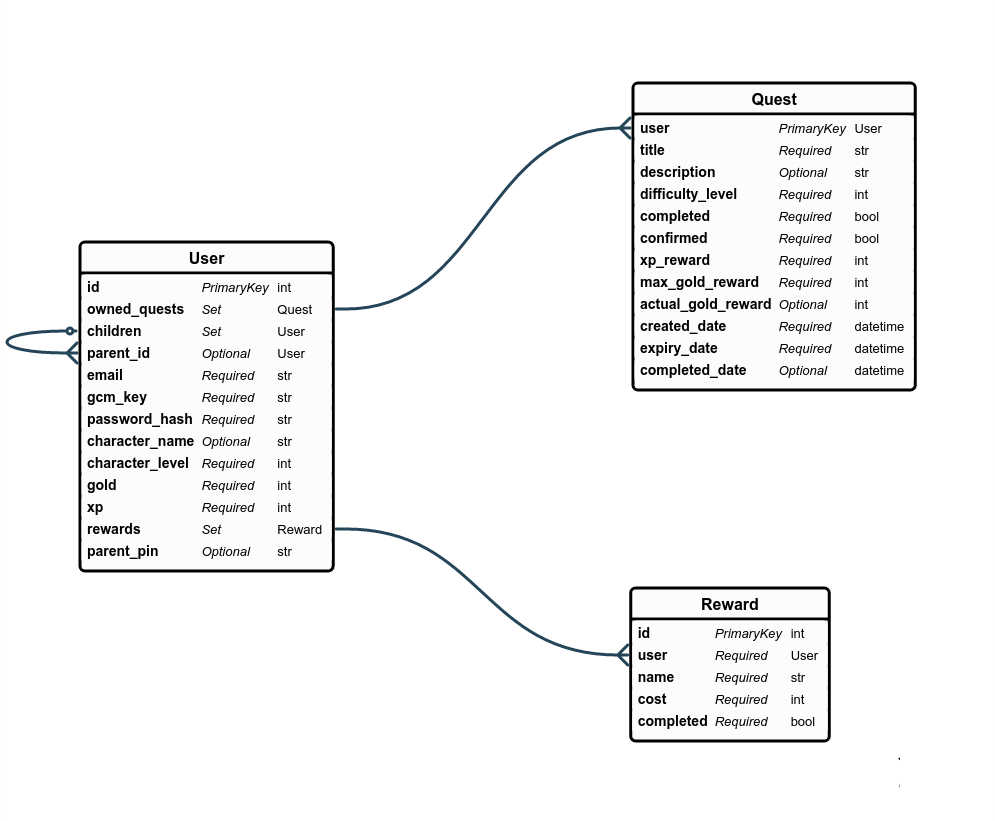
\includegraphics[scale=0.25]{images/entityRelationshipDiagram.png}
	\caption{Server Entity Relationship Diagram}
	\label{fig:erd}
\end{figure} 

\subsection{Database Access}
In this design, the central database is only accessible via the server API, rather than using a direct connection to any of the users' individual devices.
Instead, the server will offer publicly available web services that will provide functionality to input or update data. 
This has the benefit of allowing me to properly validate and sanitize any data sent by the user before being added to the database and correctly reject requests that are unsuitable. 
These services will ensure the user making the request is authorized to take actions on that account - i.e. The user making the request must be either the owner of that account or a registered parent of the user - before allowing them to perform any functionality.
This segregation of the database helps to protect user data, as the database is not made accessible over the web at any point and is therefore less vulnerable to malicious entry.

\section{Development Methodologies}
\subsection{Agile}
As I am a single developer working on this project, this is beneficial to me as it helps give early sight of potential design issues early in the project.

\section{Development Processes}
There are also many sub-processes that are born out of or tie into Agile which could be beneficial for my project.

\subsection{Test-Driven Development}
From the various development processes I have examined, I have chosen to use test-driven development as my key driving force 

However, it must also be considered that if the practice offers a higher quality of code it is inherently likely to produce less errors and therefore the productivity/time trade-off may be worth it.
It is also noted that I must be prepared as I am unfamiliar with TDD myself, and will likely experience a similar drop in productivity as I begin to practice the methodology, however the paper offered several useful tips for developers/teams who are new to the practice.

\subsection{Behaviour-Driven Development}
After planning out the requirements, the next step in the design of KidQuest was to plan out the database structure.
I created an entity relationship to map out the various tables needed and the relationships between them.

\begin{figure}[t]
	\centering
	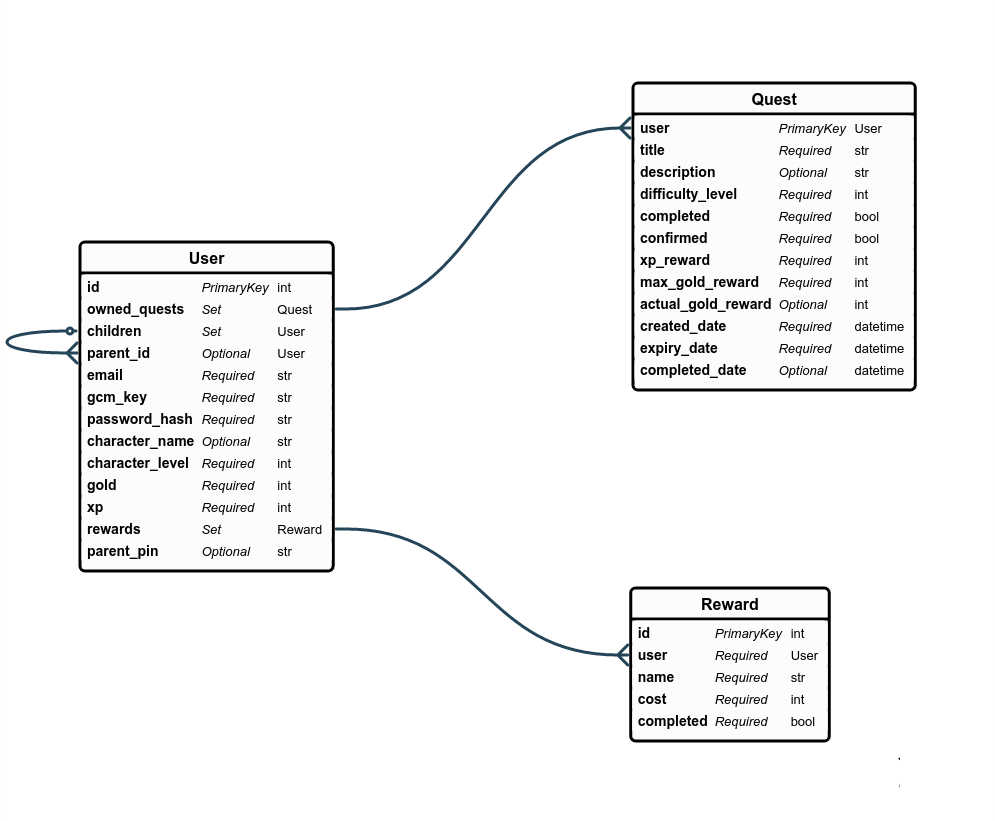
\includegraphics[width=0.75\textwidth]{images/entityRelationshipDiagram.png}
	\caption{Entity-Relationship Diagram}
	\label{fig:ERD}
\end{figure}

I have chosen to create the application in the Android SDK largely due to my previous experience with Java and Android. 
Furthermore, I believe Android is more applicable to the target audience of the app, as Android owns 82.8\% of the smartphone market share as of 2015.
%http://www.idc.com/prodserv/smartphone-os-market-share.jsp
I believe that parents are also more likely to buy their children Android phones than other brands due to the lower price point, making them more appealing when considering the likelihood of them being lost or broken by a child.

For the data analytics, I have opted to use web services written in Flask microframework for python, hosted on a server running Ubuntu Server 14.04. 
I have chosen python due to it's strong backing and community support in data analytics, and is one of the main languages of choice for scientists and statisticians.
The flask framework was chosen specifically as it is very simple to write and host RESTful APIs over the web.

To safely store and version control the code, I used a GitHub private repository to host my code in cloud storage. 
This allows me to better manage changes to the code-base. 

\section{Development Style}

\section{Testing}
Unfortunately, when developing a REST API, it is difficult to manually write and send the request to the API to test it.
Programs and scripts exist to ease the process somewhat, but I found the easiest way to be automating the requests entirely. 
As a main principle of REST is to plan out the specific endpoints that can be messaged, it becomes rather simple to plan out tests in the form of sending an example of a valid and invalid request of each request type to each endpoint.
For example, the endpoint of `/api/users/<userId>/' allows two request types, GET and PUT, which generates four test cases.
\begin{itemize}
	\item{Valid GET}
	\item{Invalid GET}
	\item{Valid PUT}
	\item{Invalid put}
\end{itemize}  
%TODO: Research what test generation this is

However, this raises issues when considering that a request could be invalid for multiple reasons, and simply testing for invalid/valid may not reach adequate code coverage.
An example of this could be that a PUT request may be invalid due to an email address already existing within the database or because they have not included a valid did not include any new data about the user, which are two separate sections of the code that arguably each require their own tests.
Because of this, it must be analysed whether or not the test cases achieve sufficient code coverage, rather than just relying on the entry points into the software.
Luckily, the python package `coverage.py' allows for simple analysis of unit tests to determine the current code coverage for tests, which will provide a higher rate of confidence.

\subsection{Unit Testing} 
Unit Testing is integral to the workflow of test-driven development

\subsection{Integration Testing}
Integration testing encompasses tests that specifically test that the various parts of the project work together correctly.
For example, integration tests for KidQuest would test that the server and mobile app are able to correctly function together, by ensuring that the app can correctly send requests and that the server receives those requests as they were sent.


\subsection{Black Box Testing}

\subsection{White Box Testing}


\subsection{Regression Testing}
Regression testing is the practice of retesting the previously tested parts of the software to ensure that they are still performing correctly after a change elsewhere in the code, it can also be used to describe the process of testing previously detected and fixed bugs to determine that they have not reappeared.
This is made significantly easier by the implementation of strong automated unit tests, which allow me to quickly retest the majority of the code by rerunning the test suite.
I also intend to follow a common development practice where a unit test is added for each defect that is found within the code, a new unit test is added to detect the presence of that bug specifically. 
This will allow me to easily spot any recurrences of legacy bugs that would otherwise go unnoticed.

\section{User Interface}
\subsection{Navigation}
A focus must be put on the usability of the screens in KidQuest.
They should not only be easy to use, but easy to learn and navigate between, and should offer minimal resistance in the use of the application.

\cite{stone2005user} classifies a good user interface design as an `easy, natural and engaging interaction between a user and a system'.

\subsection{Android Developer Guidelines}

\subsection{Wireframes}
Wireframing is a useful tool to plan out the aesthetic design of screens and the UI elements used within them. 
A wireframe is also useful to get a better overview of the navigation between screens, as they can be used to plan out the button presses that will select the next screen.
The wireframes shown in appendix \ref{appendix:wireframes} give an overview of the general aesthetic style that will be used.